\documentclass[11pt]{article}
\usepackage{amsmath, amssymb, amsthm}
\usepackage[retainorgcmds]{IEEEtrantools}

\usepackage[pdftex]{graphicx}
\usepackage{tikz}
\usetikzlibrary{intersections}
\usepackage{circuitikz}

\usepackage{fancyhdr}

%Listings stuff
\usepackage{listings}
\usepackage{lstautogobble}
\usepackage{color}

\definecolor{gray}{rgb}{0.5,0.5,0.5}
\lstset{
basicstyle={\small\ttfamily},
tabsize=3,
numbers=left,
numbersep=5pt,
numberstyle=\tiny\color{gray},
stepnumber=2,
breaklines=true,
boxpos=t
}

%Format stuff
\pagestyle{fancy}
\headheight 35pt

%Header info
\chead{\Large \textbf{Phasor Analysis of AC Circuits}}
\lhead{}
\rhead{}

\begin{document}
\section{Basic Principles}
	A \textbf{phasor} is a geometric vector representation of a sinusoidal function with constant amplitude multiplier, frequency, and phase. It is represented as a vector in the imaginary plane that rotates around the origin at a constant frequency. Phasors can be used in the analysis of AC circuits because power sources supply an oscillating voltage at a constant frequency.
	
	For the following analyses, assume that the voltage supplied from the source is a simple harmonic function.
	\begin{equation}
		V_S = V_0 e^{i\omega t}
	\end{equation}
	
	\subparagraph{Resistors} Current and voltage across a resistor are in phase as long as the resistance is real.
		\begin{IEEEeqnarray}{rCl}
			V_R & = & IR\\
		\end{IEEEeqnarray}
		
	\subparagraph{Capacitors} Current and voltage across a capacitor are exactly $\pi/4$ out of phase, with the capacitor voltage lagging behind the current.
		\begin{IEEEeqnarray}{rCl}
			Q & = & CV\\
			I & = & \dot{Q} = C\frac{dV}{dt}\\
			I & = & i\omega CV_0 e^{i\omega t}\\
			V & = & I\left(\frac{1}{i \omega C}\right)\\
			X_C & = & \frac{1}{i \omega C}\\\nonumber\\
			V & = & IX_C
		\end{IEEEeqnarray}
		
	\subparagraph{Inductors} Current and voltage across an inductor are exactly $\pi/4$ out of phase, with the inductor voltage ahead of the current.
		\begin{IEEEeqnarray}{rCl}
			V & = & L\frac{dI}{dt}\\
			I & = & \frac{1}{i\omega L}(V_0e^{i\omega t})\\
			V & = & I(i\omega L)\\
			X_L & = & i\omega L\\
			V & = & IX_L
		\end{IEEEeqnarray}
		
\section{Driven RL Circuits}
	\begin{center}
	\begin{circuitikz}
		\draw (0, 0) to[vsourcesin] (0, 3) -- (2, 3) to[R] (2, 1) to[C] (2, 0) -- (0, 0);
	\end{circuitikz}
	\end{center}
	
	The phasor diagram for a driven RL circuit looks like the following:
	\begin{center}
	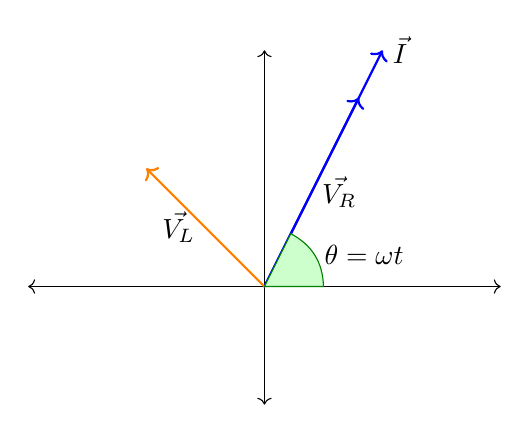
\begin{tikzpicture}
		[scale=1.5,line cap=round,
		%Styles
		axes/.style=,
		important line/.style={very thick},
		information text/.style={rounded corners,fill=red!10,inner sep=1ex},
		dot/.style={circle,inner sep=1pt,fill,label={#1},name=#1}			
		]
		
		%Colors
		\colorlet{anglecolor}{green!50!black}	%angle arcs/lines
		
		%The graphic
		\begin{scope}[axes]
			\draw[<->] (0, -1) -- (0, 2);
			\draw[<->] (-2, 0) -- (2, 0);
		\end{scope}
		
		\coordinate (l) at (-1, 1);
		\coordinate (s) at (1, 2);
		
		\draw[->,blue,thick] (0, 0) -- (s) node[right,black]{$\vec{I}$};
		\draw[->,blue,thick] (0, 0) -- node[right,black]{$\vec{V_R}$} (.8, 1.6);
		\draw[->,orange,thick] (0,0) -- node[left,black]{$\vec{V_L}$}(l);
		
		\filldraw[fill=green!20, draw=anglecolor] (0, 0) -- ($(0,0)!5mm!(s)$) to[bend left] node[right,black]{$\theta = \omega t$}(5mm,0mm) -- cycle;
	\end{tikzpicture}
	\end{center}
	
	From Kirchoff we know that $V_S = V_R + V_L$. Now we can use phasors to solve the system geometrically instead of algebraically. Consider the following phasor system determined from Kirchoff's rules:
	
	\begin{center}
	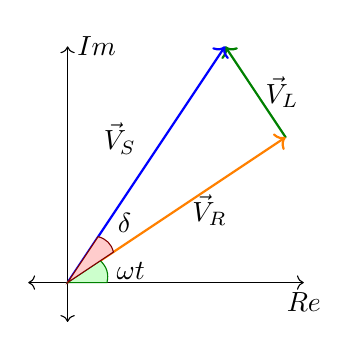
\begin{tikzpicture}
		[scale=1,line cap=round,
		%Styles
		axes/.style=,
		important line/.style={very thick},
		information text/.style={rounded corners,fill=red!10,inner sep=1ex},
		dot/.style={circle,inner sep=1pt,fill,label={#1},name=#1}			
		]
		
		%Colors
		\colorlet{anglecolor}{green!50!black}	%angle arcs/lines
		
		%The graphic
		\begin{scope}[axes]
			\draw[<->] (0, -.5) -- (0, 3) node[right]{$Im$};
			\draw[<->] (-.5, 0) -- (3, 0) node[below]{$Re$};
		\end{scope}
		
		\coordinate (s) at (2, 3);
		\coordinate (l) at ($(0,0)!(s)!(3,2)$);
		
		\draw[anglecolor,->,thick] (l) -- node[right,black]{$\vec{V}_L$} (s);
		\draw[blue,->,thick] (0,0) -- node[above left,black]{$\vec{V}_S$} (s);
		\draw[orange,->,thick] (0,0) -- node[right=2pt,black]{$\vec{V}_R$}(l);
		
		\filldraw[fill=green!20,draw=anglecolor] (0,0) -- ($(0,0)!5mm!(l)$) to[bend left] node[right,black]{$\omega t$}(5mm, 0) -- cycle;
		
		\filldraw[fill=red!20,draw=red!50!black] (0,0) -- ($(0,0)!7mm!(l)$) to[bend right] node[above right,black]{$\delta$} ($(0,0)!7mm!(s)$) -- cycle;
	\end{tikzpicture}
	\end{center}	
	
	\begin{IEEEeqnarray}{rCl}
		\vec{V}_S & = & \vec{V}_R + \vec{V}_L\\
		|\vec{V}_S| & = & V_0 = \sqrt{V_R^2 + V_L^2}\\
		|\vec{V}_R| & = & I_0 R\\
		|\vec{V}_L| & = & I_0 \omega L
	\end{IEEEeqnarray}
	
	This yields the following solution
	\begin{equation}
		V_0 = I_0 \sqrt{R^2 + (\omega L)^2}
	\end{equation}
		
	To make the solution look more like Ohm's law, define the \textbf{impedance} of the system as
	\begin{equation}
		Z = \sqrt{R^2 + (\omega L)^2}
	\end{equation}
	which turns the solution to
	\begin{equation}
		V_0 = I_0 Z
	\end{equation}
	
	To calculate the phase difference $\delta$, since $\vec{V}_L \perp \vec{V}_R$, the phasor diagram is a rotating right triangle.
	\begin{equation}
		\delta = \tan^{-1}\left(\frac{V_L}{V_R}\right) = \tan^{-1} \left(\frac{\omega L}{R}\right)
	\end{equation}
	
\section{Driven RLC Circuits}
	\begin{center}
	\begin{circuitikz}[scale=0.75]
		\draw (0,0) to[vsourcesin] (0,4) -- (1, 4) to[R] (3,4) -- (3,3) to[L] (3,0) to[C] (0,0);
	\end{circuitikz}
	\end{center}
	
	The phasor diagram for a driven RLC circuit looks like the following:
	\begin{center}
	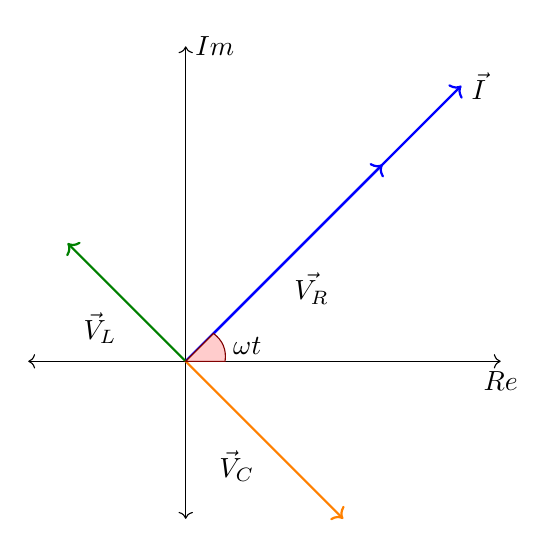
\begin{tikzpicture}
		[scale=1,line cap=round,
		%Styles
		axes/.style=,
		important line/.style={very thick},
		information text/.style={rounded corners,fill=red!10,inner sep=1ex},
		dot/.style={circle,inner sep=1pt,fill,label={#1},name=#1}			
		]
		
		%Colors
		\colorlet{anglecolor}{green!50!black}	%angle arcs/lines
		
		%The graphic
		\begin{scope}[axes]
			\draw[<->] (-2,0) -- (4, 0) node[below]{$Re$};
			\draw[<->] (0, -2) -- (0, 4) node[right]{$Im$};
		\end{scope}
		
		\draw[blue,thick,->] (0, 0) -- (3.5,3.5) node[right,black]{$\vec{I}$};
		\draw[blue,thick,->] (0,0) -- node[below right,black]{$\vec{V_R}$} (2.5,2.5);
		
		\draw[orange,thick,->] (0,0) -- node[below left,black]{$\vec{V}_C$}(2, -2);
		\draw[anglecolor,thick,->] (0,0) -- node[below left,black]{$\vec{V}_L$} (-1.5, 1.5);
		
		\filldraw[fill=red!20,draw=red!50!black] (0,0) -- ($(0,0)!5mm!(1,1)$) to[bend left] node[right,black]{$\omega t$} (.5, 0) -- cycle;
	\end{tikzpicture}
	\end{center}
	
	From Kirchoff's rules, we know that $V_S = V_R + V_L + V_C$. Because $\vec{V}_C$ and $\vec{V}_L$ are exactly $\pi$ out of phase, we can create the following phasor system:

%	\begin{center}
%	\begin{tikzpicture}
%		[scale=3,line cap=round,
%		%Styles
%		axes/.style=,
%		important line/.style={very thick},
%		information text/.style={rounded corners,fill=red!10,inner sep=1ex},
%		dot/.style={circle,inner sep=1pt,fill,label={#1},name=#1}			
%		]
%		
%		%Colors
%		\colorlet{anglecolor}{green!50!black}	%angle arcs/lines
%		
%		%The graphic
%	\end{tikzpicture}
%	\end{center}

%	\begin{figure}[htb]
%		\centering
%		\includegraphics[width=0.8\textwidth]{filename.eps}
%		\caption{Caption.}
%		\label{fig:figure}
%	\end{figure}

%		\def\enotesize{\normalsize}
%		\theendnotes
\end{document}